\documentclass[12pt]{article}
\usepackage[top=1in, bottom=1in, left=1in, right=1in]{geometry}

\usepackage{setspace}
\onehalfspacing

\usepackage{amssymb}
%% The amsthm package provides extended theorem environments
\usepackage{amsthm}
\usepackage{epsfig}
\usepackage{times}
\renewcommand{\ttdefault}{cmtt}
\usepackage{amsmath}
\usepackage{graphicx} % for graphics files

% Draw figures yourself
\usepackage{tikz} 

% writing elements
\usepackage{mhchem}

% The float package HAS to load before hyperref
\usepackage{float} % for psuedocode formatting
\usepackage{xspace}

% from Denovo Methods Manual
\usepackage{mathrsfs}
\usepackage[mathcal]{euscript}
\usepackage{color}
\usepackage{array}

\usepackage[pdftex]{hyperref}
\usepackage[parfill]{parskip}

% math syntax
\newcommand{\nth}{n\ensuremath{^{\text{th}}} }
\newcommand{\ve}[1]{\ensuremath{\mathbf{#1}}}
\newcommand{\Macro}{\ensuremath{\Sigma}}
%---------------------------------------------------------------------------
%---------------------------------------------------------------------------
\begin{document}
\begin{center}
{\bf NE 250, F15 \\
Introduction and Background \\ August 26, 2015}
\end{center}

\setlength{\unitlength}{1in}
\begin{picture}(6,.1) 
\put(0,0) {\line(1,0){6.25}}         
\end{picture}

\noindent \textbf{Syllabus}

Fundamentally, we're learning about Nuclear Reactor Theory--but what does that mean? 
We're concerned about producing energy through nuclear reactions.
Neutrons can interact with large, unstable nuclei and one of the outcomes of such an interaction is fission.
Fission releases a great deal of energy, which can be captured and used to produce electricity.
The neutrons can also cause reactions other than fission.

The neutron balance, or neutron ``economy", is what we're interested in learning how to monitor and control. 
We must design reactors to balance production and loss.
(1) Determining the probabilities of neutron-nuclear reactions and (2) the derivation and solution of an equation that uses these probabilities is the focus of this course.

How you use the liberated energy to produce electricity is beyond this course: heat transfer, fluid flow, structural and materials analysis, and power systems. 
All of this affects the neutronics (and incorporating these components is a large area of research), but will generally be out of scope for this class.

To discover for yourselves what is the science of neutronics...

Go through syllabus in detail.

Integrity.

Cover topics and talk about why we care about learning any of that stuff.

Show bCourses and resources page; explain how I'll use the page.

Chapters 1-3 of Duderstadt and Hamilton should be known or reviewed.

Next week I will be out of town. 
Monday and you will have a literature review class at the engineering library with Lisa Ngo. 
Engineering Library Training Room at 10.  

Researcher Richard Vasques will lecture on Wednesday, 9/2.

\clearpage
%---------------------------------------------------------------------------
\section*{Nuclear Physics of Physics Chain Reactions}
To begin determining probabilities of neutron-nuclear reactions, we will first review the aspects of nuclear physics that are relevant for fission chain reactions. 

\subsection*{Reactions}
There are two types of reactions
\begin{enumerate}
\item spontaneous disintegration
\item induced by collision.
\end{enumerate}

Notation reminder: \ce{^{A}_{Z}X} indicates that chemical element $X$ has $Z$ protons (atomic number) and $A$ total nucleons (protons + neutrons; mass number).\\
Note that this leaves $N$ neutrons.\\
Excited states are written as \ce{^{A}_{Z}X^*}, and metastable/isomeric as \ce{^{A}_{Z}X^m}.

Spontaneous reactions are things like $\alpha$, $\beta$, and $\gamma$ decay.\\
These are probabilistic events that depend only on the type of nucleus.

$\lambda$ is the decay constant. If $N(t)$ is the number of nuclei at $t$ and $N_0$ is the original number of nuclei, then
%
\begin{align*}
N(t + dt) - N(t) &= -\lambda N(t) = dN(t)\\
-\frac{dN}{dt} &= \lambda N(t)\\
N(t) &= N_0 e^{-\lambda t}
\end{align*}

The rate of decay is\[\lambda N_0 e^{-\lambda t} \:.\]

The probability that a given nucleus will decay in a given time interval is \[p(t) dt = \lambda e^{-\lambda t} dt \:.\]

We are interested in the mean lifetime of nuclei (predicting the decay of a particular nucleus doesn't really work)
\[\bar{t} \equiv \int_0^\infty dt \: t \: p(t) - \lambda \int_0^\infty dt \: t \: e^{-\lambda t} = \frac{1}{\lambda} \:. \]
We very often use the related quantity of half-life (time it takes for half of the original nuclei to decay) 
\[t_{\frac{1}{2}} = \frac{\ln(2)}{\lambda} \:. \]

\subsection*{Nuclear Collision Reactions}
Induced reactions generally involve a projectile and a target. \\
For us, the projectile is usually a neutron and induced reactions fall into the categories of scattering or absorption.\\
Within scattering there is elastic (KE conserved) or inelastic (some KE is lost and given up later).\\
Absorption can result in all sorts of outcomes. 
A compound nucleus is formed and particles are emitted: (n, fission), (n, 2n), (n, $\gamma$), and so on.
%
\begin{itemize}
\item radiative capture: n + \ce{^A_Z X} $\rightarrow$ (\ce{^{A+1}_Z X^*}) $\rightarrow$ \ce{^{A+1}_Z X} + $\gamma$
\item (n, 2n): n + \ce{^A_Z X} $\rightarrow$ \ce{^{A-1}_Z X} + 2n
\item fission: n + \ce{^A_Z X} $\rightarrow$ fission products + 1-5 neutrons + 200 MeV
\end{itemize}

In these interactions, mass often changes and we can use Einstein's famous formula to get the energy required or released:
\begin{align*}
a + b &\rightarrow c + d\\
Q &= \bigl[ (m_a + m_b) - (m_c + m_d) \bigr]c^2
\end{align*}

Any of these interactions are \textbf{probabilistic}, and the probabilities are expressed as cross sections. \\
We will use $\sigma$ for microscopic and $\Sigma$ as macroscopic.\\
The reaction rate [\# / cm$^2$ s] = $\phi \sigma N$ = $nv \sigma N$.

A cross section is a physical quantity that can be measured (caveat about the data we actually have).\\
The value depends on the nuclide, the reaction, neutron energy, and temperature of the target. \\
Cross sections are measured in barns, $10^{-24}$ cm$^2$.

Cross sections have features that can be difficult to calculate or model accurately, for example, resonances.\\
Resonances come from energy levels within the target nucleus. \\
If the energy of the incoming particle and the binding energy of it being added to the nucleus line up with an internal energy level, the reaction is much more likely.\\

The interaction probabilities depend on the relative speed between particles.\\
However, the target is moving and this ``broadens" the probability and slightly shifts the relative speed.\\
This is a doppler shift / doppler broadening.\\
The cross section peak gets wider and lower with increasing temperature (speed).\\
The total area under the curve remains constant (total probability of interaction is unchanged).

Calculating cross sections and doppler-broadened cross sections is an important and non-trivial task.

\begin{center}
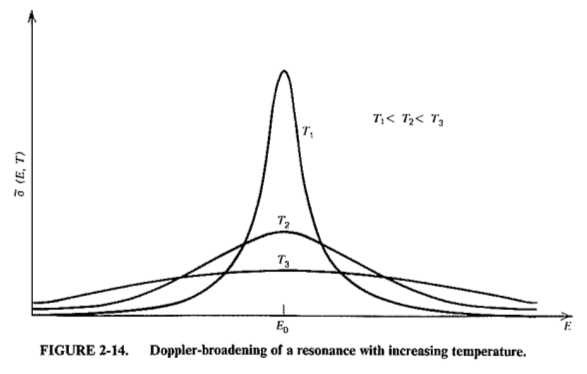
\includegraphics[height=2.5 in]{../figs/doppler}
\end{center}






\end{document}

